% Beamer template for presentations of LIDET members
%
% Author: Luiz C. Vieira
% version: 2

% The default aspect ratio is 4:3, but it can be changed to 16:9 (more interesting for
% widescreen projections) if the parametre `aspectration=169' is added to the document
% class as above.
%\documentclass[table, usenames, svgnames, dvipsnames, aspectratio=169]{beamer}

% NOTE: This is currently done automatically through the Makefile! There are two
%       targets, one called ``full'' and the other called ``wide'' - the former
%       builds the presentation to 4:3 (fullscreen) and the latter to 16:9 (widescreen).
%       So, use ``make full'' or ``make wide'' instead of changing the aspect ration through
%       here! The target ``all'' calls by default the target ``wide''.
\providecommand\classopts{}
\expandafter\documentclass\expandafter[table, usenames, svgnames, dvipsnames, \classopts]{beamer}

\usepackage{etex}
\usepackage{beamerthemeshadow}
\usepackage[english]{babel}
\usepackage[latin1]{inputenc}
\usepackage[absolute,overlay]{textpos}
\usepackage{array}
\usepackage{framed}
\usepackage{booktabs}
\usepackage{caption}
\usepackage{subcaption}
\usepackage{outlines}
\usepackage{ulem}
\usepackage{xcolor,colortbl}
\usepackage{ragged2e}
\usepackage{tikz}

% ---------------------------------------------------------------------------- %
% Presentation definitions
% ---------------------------------------------------------------------------- %
\usetheme{Luebeck}
\hypersetup{pdfpagemode=FullScreen} % Starts the presentation in full screen

% layout
\setbeamerfont{frametitle}{size=\normalsize}
\setbeamerfont{title}{size=\normalsize}
\beamertemplatenavigationsymbolsempty
\setbeamertemplate{bibliography item}[text]%

% colors
\definecolor{lidet_orange}{rgb}{0.9, 0.49, 0.09}
\definecolor{lidet_black}{rgb}{0.2, 0.2, 0.2}

\setbeamercolor{title}{bg=lidet_orange}
\setbeamercolor{structure}{bg=white, fg=lidet_orange}
\setbeamercolor{normal text}{fg=black}
\setbeamercolor{section in head/foot}{fg=white, bg=lidet_black}
\setbeamercolor{postit}{fg=white, bg=lidet_orange!90!lidet_black}

% shadow
\makeatletter
\pgfdeclareverticalshading[black,bg]{bmb@shadow}{200cm}{%
  color(0bp)=(lidet_black!25); color(4bp)=(black!50!bg); color(8bp)=(black!50!bg)}
\pgfdeclareradialshading[black,bg]{bmb@shadowball}{\pgfpointorigin}{%
  color(0bp)=(black!50!bg); color(4bp)=(lidet_black!25)}
\pgfdeclareradialshading[black,bg]{bmb@shadowballlarge}{\pgfpointorigin}{%
  color(0bp)=(black!50!bg); color(4bp)=(black!50!bg); color(8bp)=(lidet_black!25)}
%
\makeatother

% Captions for images and tables
\setlength{\abovecaptionskip}{5pt plus 5pt minus 5pt}
\setlength{\belowcaptionskip}{5pt plus 5pt minus 5pt}
\captionsetup[figure]{font=scriptsize,labelfont=scriptsize}
\captionsetup[table]{font=scriptsize,labelfont=scriptsize}
\captionsetup{labelformat=empty,labelsep=none}

% Dimensions for table rules
\setlength\heavyrulewidth{0.1em} 
\setlength\lightrulewidth{0.01em}
\setlength\belowrulesep{0.10ex}
\setlength\aboverulesep{0.10ex}

% Define macros to mark the begining and ending of references
% Basically, handles the automatically spanned frames (due to parameter allowframebreaks)
% as backup frames, so they do not influence in the frame numbering
\newcommand{\referencesbegin}{
   \newcounter{framenumberappendix}
   \setcounter{framenumberappendix}{\value{framenumber}}
}
\newcommand{\referencesend}{
   \addtocounter{framenumberappendix}{-\value{framenumber}}
   \addtocounter{framenumber}{\value{framenumberappendix}} 
}

% Section frames (that appear before each section)
\AtBeginSection[] 
{
	{
		\setbeamertemplate{footline}{} % Hide the footline locally for these frames
		\begin{frame}<beamer>[noframenumbering]
			\begin{center}
				\begin{tikzpicture}
					\node[align=left, left color=lidet_orange, right color=lidet_orange, draw, rounded corners, minimum width=10cm, minimum height=1cm] {\color{white} \textbf{\insertsectionhead}};
				\end{tikzpicture}
			\end{center}
			\footnotesize{ \tableofcontents[currentsection, hideothersubsections] }
		\end{frame}
	}
}

\DeclareGraphicsExtensions{.pdf,.jpg,.png}
\graphicspath{{./images/}}

% ---------------------------------------------------------------------------- %
% Presentation title, author and institution
% ---------------------------------------------------------------------------- %
\title{\textbf{Presentation Title}}
\subtitle{{\small Presentation Subtitle}}

\author[Author's Name]{\scriptsize
    Author's Name\\
    author.email@ime.usp.br
}

\institute[LIDET (IME - USP)]{\\[1.0mm] 
MSc/PhD Student\\
Department of Computer Science}

\date{{\tiny Presentation Date}}

% ---------------------------------------------------------------------------- %
% Presentation content
% ---------------------------------------------------------------------------- %

% ---------------------------------------------------------------------------- %
\begin{document}
% ---------------------------------------------------------------------------- %

% ---------------------------------------------------------------------------- %
% First Slide (index 0) = cover
% ---------------------------------------------------------------------------- %

{%\usebackgroundtemplate{}} 
\begin{frame}[plain, noframenumbering]

	\begin{columns}[c]
		\column{0.2\textwidth}
			\hspace*{-1.5em}
			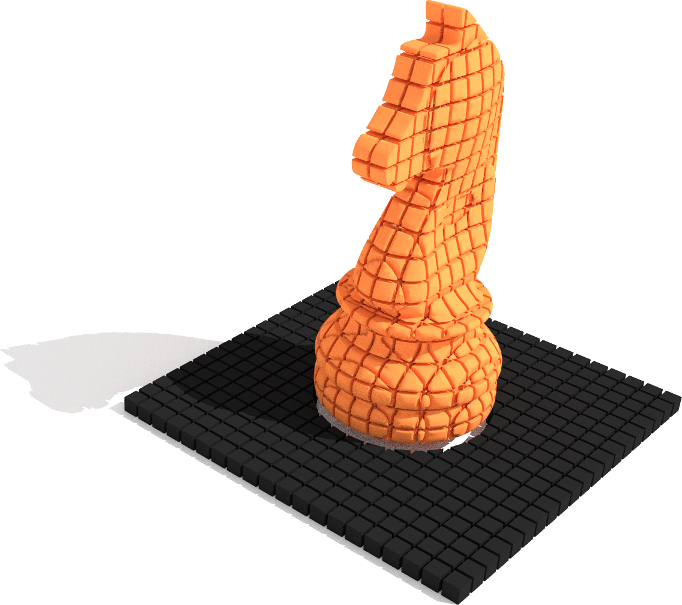
\includegraphics[width=0.35\paperwidth]{side_bar}\\
		\column{0.01\textwidth}
		\column{0.70\textwidth}
			\titlepage
			\hspace*{+0.5em}
			\begin{center}
				
\includegraphics[height=1.0cm]{lidet-logo}\\
				
\includegraphics[height=1.0cm]{ime-logo}\\
			\end{center}
	\end{columns}
	%\addtocounter{framenumber}{-1}
\end{frame}
}

% ---------------------------------------------------------------------------- %
% Other Slides (index from 1 onwards)
% ---------------------------------------------------------------------------- %

% setup navigation symbols and footline
\setbeamertemplate{navigation symbols}{}
\setbeamertemplate{footline}{
   \begin{beamercolorbox}[ht=4ex,leftskip=.3cm,rightskip=.3cm]{author in head/foot}
    %\usebeamercolor{lidet_orange}
    \hrule
    \vspace{0.1cm}
    \insertdate \hfill \insertframenumber/\inserttotalframenumber \newline
    \insertshortauthor \ - \inserttitle \hfill \insertshortinstitute
   \end{beamercolorbox}
   \vspace*{0.1cm}
} 

% ---------------------------------------------------------------------------- %
\begin{frame}[plain]
\frametitle{\textbf{Agenda}}

	\hspace*{+4.0em}
	\footnotesize{ \tableofcontents }
\end{frame}

% ---------------------------------------------------------------------------- %
\section{Section One}
% ---------------------------------------------------------------------------- %

\subsection{Subsection One-One}

% ------------------------------
\begin{frame}
	\frametitle{\textbf{Frame with Items}}
	
	\begin{outline}
		\1 This is the first item
			\2[-] {\scriptsize with a subitem item using a dash symbol}
			\2[-] {\scriptsize and another one}
		
		\vspace{1em}
	
		\1 This is another item
			\2[o] {\scriptsize with a subitem with a circle symbol}
			\2[x] {\scriptsize and another with a different symbol}
			\2[$\cdot$] {\scriptsize and another with a different symbol}
	\end{outline}

\end{frame}

% ------------------------------
\begin{frame}
	\frametitle{\textbf{Frame with Items (in Columns)}}
	
	\begin{columns}[c]
		\column{0.5\textwidth}
			\begin{outline}
				\1 This is the first item
					\2[-] {\scriptsize with a subitem item using a dash symbol}
					\2[-] {\scriptsize and another one}
				
				\vspace{1em}
			
				\1 This is another item
					\2[o] {\scriptsize with a subitem with a circle symbol}
					\2[x] {\scriptsize and another with a different symbol}
					\2[$\cdot$] {\scriptsize and another with a different symbol}
			\end{outline}
		
		\column{0.5\textwidth}		
			\begin{outline}
				\1 This is the first item
					\2[-] {\scriptsize with a subitem item using a dash symbol}
					\2[-] {\scriptsize and another one}
				
				\vspace{1em}
			
				\1 This is another item
					\2[o] {\scriptsize with a subitem with a circle symbol}
					\2[x] {\scriptsize and another with a different symbol}
					\2[$\cdot$] {\scriptsize and another with a different symbol}
			\end{outline}
		
	\end{columns}	

\end{frame}

\subsection{Subsection One-Two}

% ------------------------------
\begin{frame} 
	\frametitle{\textbf{Frame with Long Text}}
	
	{\small
		\justifying
		A Reading from the Book of Armaments, Chapter 4, Verses 16 to 20:
		\\[1em]
		Then did he raise on high the Holy Hand Grenade of Antioch, saying, ``Bless this, O Lord, that with it thou mayst blow thine enemies to tiny bits, in thy mercy.'' And the people did rejoice and did feast upon the lambs and toads and tree-sloths and fruit-bats and orangutans and breakfast cereals~\dots Now did the Lord say, ``First thou pullest the Holy Pin. Then thou must count to three. Three shall be the number of the counting and the number of the counting shall be three. Four shalt thou not count, neither shalt thou count two, excepting that thou then proceedeth to three. Five is right out. Once the number three, being the number of the counting, be reached, then lobbest thou the Holy Hand Grenade in the direction of thine foe, who, being naughty in my sight, shall snuff it.''
		\\[1em]
		{\scriptsize From Monty Python, ``Monty Python and the Holy Grail'' (1975)}
	}
	
\end{frame}

% ------------------------------
\begin{frame} 
	\frametitle{\textbf{Frame with Text Block}}
	
	\begin{block}{{\scriptsize Coca-Cola Ingredients}}
		{\tiny
			\begin{itemize}
				\item 28 g caffeine citrate
				\item 85 g citric acid
				\item 30 ml vanilla extract
				\item 946 ml lime juice
				\item 71 g ``Merchandise 7X'' (263 ml alcohol, 20 drops orange oil, 10 drops cinnamon oil, 30 drops lemon oil, 5 drops coriander oil, 10 drops nutmeg oil, 10 drops neroli oil)
				\item 14 kg sugar
				\item 118.3 ml fluid extract of coca leaves (flavour essence of the coca leaf)
				\item 9.5 l water
				\item caramel sufficient to give colour
			\end{itemize}
			Source: Wikipedia
		}
	\end{block}

\end{frame}

% ---------------------------------------------------------------------------- %
\section{Section Two}
% ---------------------------------------------------------------------------- %

\subsection{Subsection Two-One}

% ------------------------------
\begin{frame} 
	\frametitle{\textbf{Frame with Citations}}
	
	\begin{outline}
		\1 Interaction is a phenomenon of mutual or reciprocal influence that happens when two or more entities communicate with or react to each other \cite{Wagner1994}.
		
		\vspace{1em}
		
		\1 User Experience is a person's perceptions and responses resulting from the use and/or anticipated use of a product, system or service \cite{ISO2010}
	\end{outline}	

\end{frame}

% ------------------------------
\begin{frame} 
	\frametitle{\textbf{Frame with Figure}}

	\begin{center}
		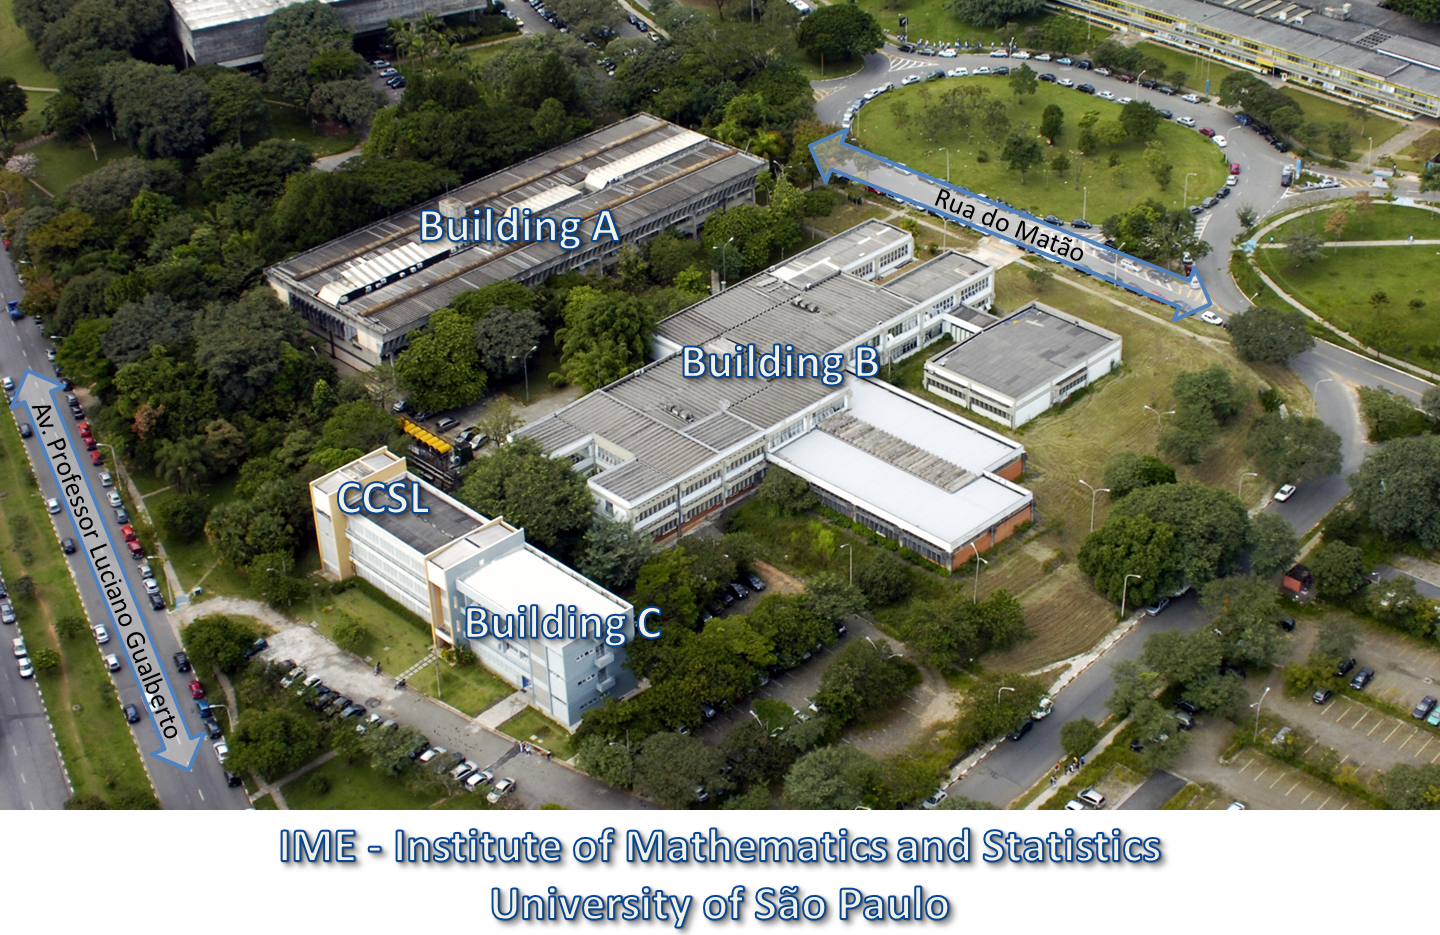
\includegraphics[height=6.5cm]{ime-usp}
	\end{center}

\end{frame}

\subsection{Subsection Two-Two}

% ------------------------------
\begin{frame} 
	\frametitle{\textbf{Frame with Figure (and Caption)}}

	\begin{figure}
		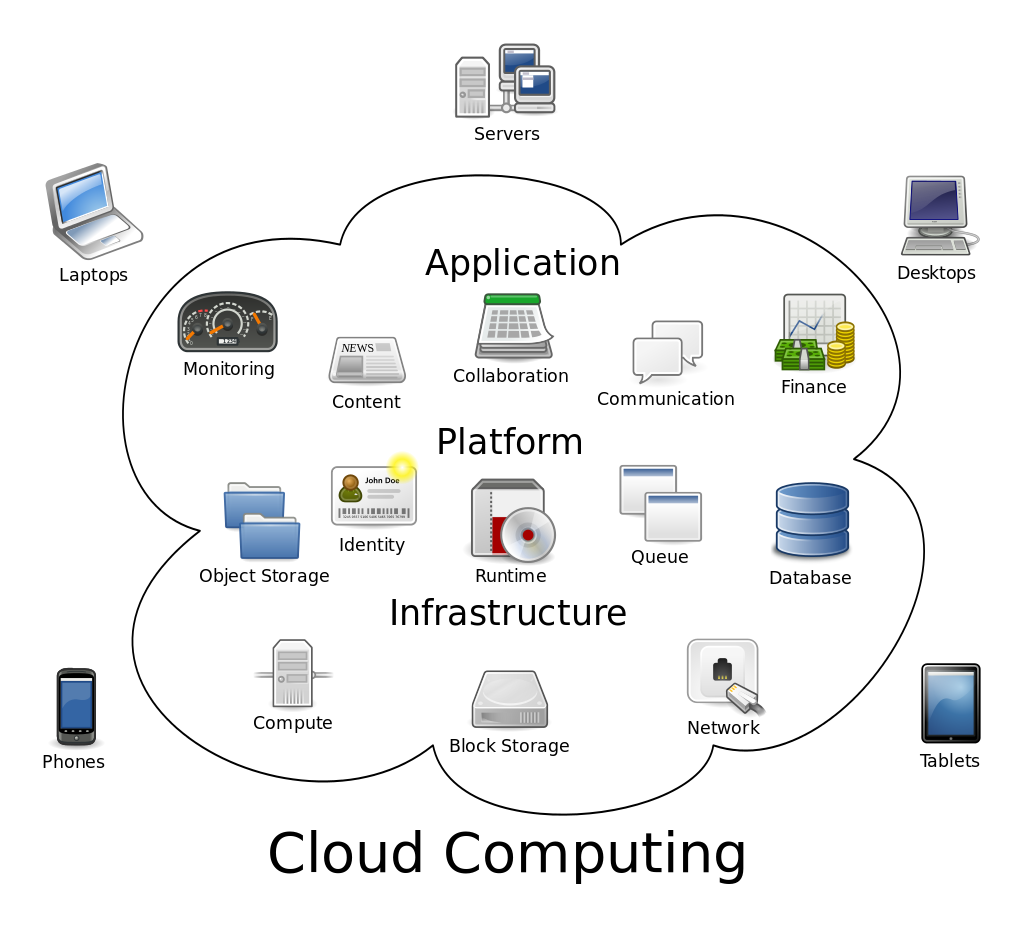
\includegraphics[height=5.5cm]{cloud-computing}
		\caption{Cloud computing metaphor. Source: Wikipedia}
	\end{figure}

\end{frame}

% ------------------------------
\begin{frame} 
	\frametitle{\textbf{Frame with Subfigures}}

    \begin{figure}
	    \centering
	    \begin{subfigure}[!h]{0.25\paperwidth}
	    	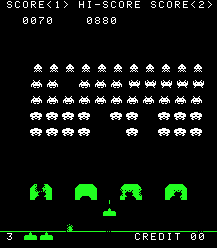
\includegraphics[width=\textwidth]{space-invaders}
	        \caption{Space Invaders (1978)}
	    \end{subfigure}
	    ~
		\begin{subfigure}[!h]{0.25\paperwidth}
	        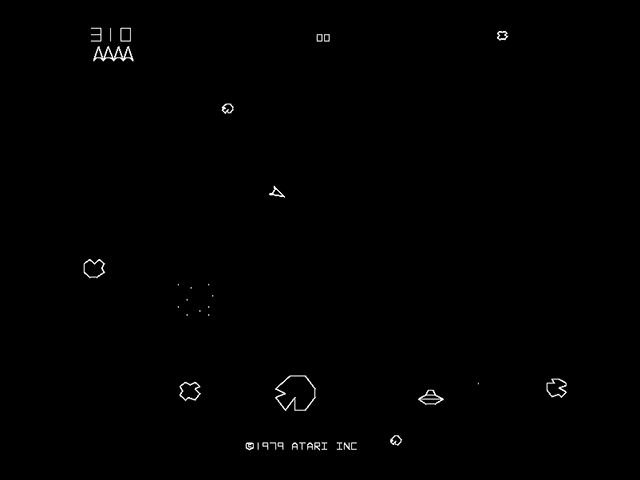
\includegraphics[width=\textwidth]{asteroids}
	        \caption{Asteroids (1979)}
	    \end{subfigure}
	    ~
	    \begin{subfigure}[!h]{0.25\paperwidth}
	        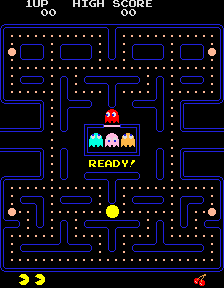
\includegraphics[width=\textwidth]{pac-man}
	        \caption{Pac-Man (1980)}
	    \end{subfigure}
	    \caption{Classic Atari arcade games. Source: Wikipedia}
    \end{figure}

\end{frame}

% ---------------------------------------------------------------------------- %
\section{Conclusion}
% ---------------------------------------------------------------------------- %

% ------------------------------
\begin{frame}
	\frametitle{\textbf{Frame with Table}}

	\begin{table}
		\caption{Some important inventors and their inventions. Source: Wikipedia}
		\begin{tabular}{c|c}
			\toprule
			\rowcolor{lidet_black}
			{\color{white} \textbf{Inventor}} & {\color{white}\textbf{Invention}}\\
			\midrule			
			{\scriptsize Alexander Graham Bell} & {\scriptsize Telephone}\\
			{\scriptsize Galileo Galilei} & {\scriptsize Telescope}\\
			{\scriptsize Johannes Gutenberg} & {\scriptsize Mechanical Printing Press}\\
			{\scriptsize Levi Strauss} & {\scriptsize Denim Trousers (Jeans)}\\
			{\scriptsize Peter Henlein} & {\scriptsize Pocket Watch}\\
			\bottomrule
		\end{tabular}
	\end{table}

\end{frame}

% ----------------------------------------
\subsection{The End}
% ----------------------------------------

% ------------------------------
\begin{frame}
	\frametitle{\textbf{C'est Fini!}}
	
	\begin{center}
		{\Huge And that is all, folks!}
	\end{center}
	
\end{frame}

% ------------------------------------------
% References
% ------------------------------------------

\referencesbegin
\begin{frame}[plain, allowframebreaks]
	\frametitle{\textbf{References}}
	\bibliographystyle{abbrv}
	{\tiny \bibliography{bibliography}}
\end{frame}
\referencesend


% ---------------------------------------------------------------------------- %
% Last Slide = cover + thanks
% ---------------------------------------------------------------------------- %

\institute{
	\begin{center}
		\LARGE{Thank you!}\\[3.0mm]
	\end{center}
}
\date{}
{%\usebackgroundtemplate{}} 
\begin{frame}[plain, noframenumbering]
	\begin{columns}[c]
		\column{0.2\textwidth}
			\hspace*{-1.5em}
			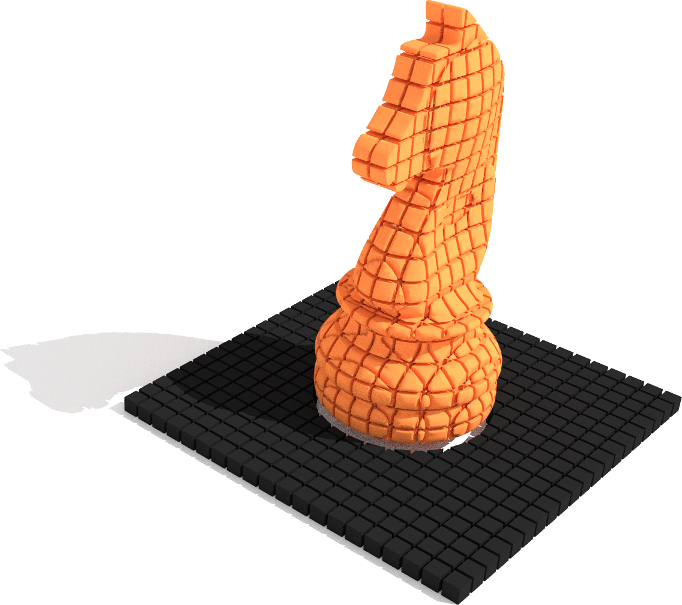
\includegraphics[width=0.35\paperwidth]{side_bar.png}
		\column{0.01\textwidth}
		\column{0.70\textwidth}
			\titlepage
			\begin{center}
				
\includegraphics[height=1.0cm]{lidet-logo}\\
				
\includegraphics[height=1.0cm]{ime-logo}\\				
			\end{center}
	\end{columns}
\end{frame}
}

\end{document}

